\documentclass[11pt]{article}
\usepackage[utf8]{inputenc}
\usepackage[russian]{babel}
\usepackage[T1]{fontenc}
\usepackage{amssymb,amsmath,clrscode,graphicx,indentfirst}

\author{Олег Смирнов}
\title{Курс kiev-clrs -- Лекция 9. Двоичные поисковые деревья}
\date{31 мая 2009 г.}

\begin{document}
\maketitle
\tableofcontents

\newpage
\setlength{\parskip}{1ex plus 0.5ex minus 0.2ex}
\section{Цель лекции}
\begin{itemize}
\item Деревья как структуры данных
\item Двоичные поисковые деревья (BST) и их связь с алгоритмом Quicksort
\item Анализ высоты рандомизированного BST
\item Алгоритмы работы с BST
\end{itemize}

\section{Деревья}

В теории графов, дерево -- связный (ориентированный или неориентированный) граф, не содержащий циклов (для любой вершины есть один и только один способ добраться до любой другой вершины). Древовидная структура -- тип организации, в котором каждый объект связан с хотя бы одним другим.

В программировании наиболее часто используются бинарные деревья, в которых число исходящих ребер не превосходит 2 и $N$-арные деревья с произвольным количеством исходящих ребер.

При хранении в памяти деревья обычно представляют в виде связной структуры, где каждый узел помимо ключа (key) хранит указатели на дочерние узлы и иногда на родительский. Для хранения $N$-арных деревьев используют структуру с левым дочерним и правым сестринским узлами (left-child, right-sibling representation). В этом случае вместо указателя на дочерние узлы каждый узел $x$ хранит два указателя:
\begin{itemize}
\item в left\_child[$x$] указатель на крайний левый дочерний узел узла $x$
\item в right\_sibling[$x$] хранится указатель на узел, расположенный на одном уровне с $x$ справа от него
\end{itemize}

\subsection{Свойства}
\begin{enumerate}
\item Дерево не имеет кратных ребер и петель.
\item Любое дерево с $n$ узлами содержит $n-1$ ребро. Более того, конечный связный граф является деревом тогда и только тогда, когда $B-P = 1$, здесь $B$ -- число узлов, $P$ -- число рёбер графа.
\item Граф является деревом тогда и только тогда, когда любые две различные его узла можно соединить единственным элементарным путём.
\item Любое дерево однозначно определяется расстояниями (длиной наименьшей цепи) между его концевыми (степени 1) узлами.
\item Любое дерево является двудольным графом. Любое дерево, содержащее счётное количество вершин, является планарным графом.
\end{enumerate}

\section{Двоичные (бинарные) поисковые деревья}
Двоичным (бинарным) поисковым деревом называется бинарное дерево, для каждого узла $x$ которого выполняется свойство:
\begin{itemize}
\item если узел $y$ лежит в левом поддереве узла $x$, то $key[y] \leqslant key[x]$
\item если узел $y$ лежит в правом поддереве узла $x$, то $key[y] \geqslant key[x]$
\end{itemize}

``Хорошими'' считаются сбалансированные бинарные деревья с высотой порядка $O(\lg n)$. У несбалансированных бинарных деревьев высота может достигать $n$. Время прохода по бинарному дереву пропорционально его высоте. Цель -- построить бинарное дерево с высотой порядка $O(\lg n)$ в большинстве случаев. Один из способов -- рандомизация, рассматривается в данной лекции.

\subsection{Сортировка массива}
Бинарные деревья поиска можно использовать для сортировки массива:
\begin{codebox}
\li $T \gets \emptyset $
\li \For $i \gets 1$ \To $n$
\li \Do Tree\_Insert($T$, $A[i]$)
  \End
\li Inorder\_Tree\_Walk(root$[T]$)
\end{codebox}

\begin{figure}[ht]
  \centering
  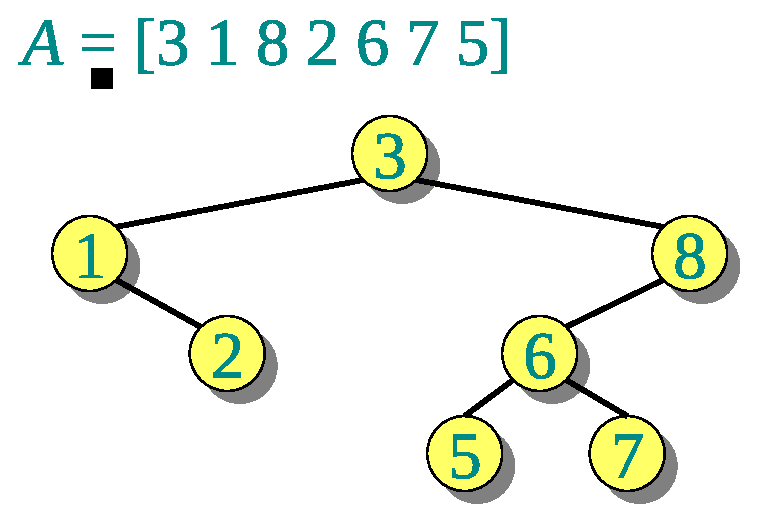
\includegraphics[width=2in]{lecture9/bs_tree.eps}
  \caption{Дерево работы BST sort}
  \label{fig:bs_tree}
\end{figure}

Время работы алгоритма складывается из частей:
\begin{itemize}
\item $O(n)$ для обхода Inorder\_Tree\_Walk
\item $\Omega(n \lg n)$ для Tree\_Insert в среднем и в лучшем случае (идеально сбалансированное бинарное дерево)
\item $T = \sum_{x \in T} depth(x) = \Theta(n^2)$ для Tree\_Insert в худшем случае (массиво уже отсортирован)
\end{itemize}

Поведение алгоритма похоже на поведение сортирвки Хоара -- Quicksort.

\section{BST и сортировка Хоара}
Алгоритмы BST sort и Quicksort выполняют одинаковое количество сравнений, но в различном порядке.
\begin{figure}[ht]
  \centering
  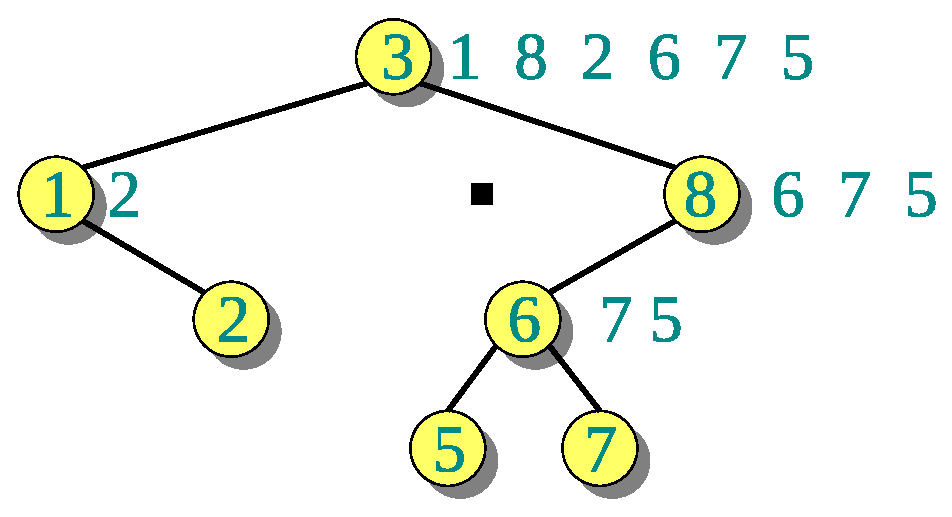
\includegraphics[width=2in]{lecture9/qs_tree.eps}
  \caption{Дерево работы Quicksort}
  \label{fig:qs_tree}
\end{figure}

Полученное дерево в точности совпадает с построенным в предыдущем примере.

Анализируя работу, можно увидеть, что алгоритм Quicksort в начале делает сравнение всех элементов с первым опорным (3), генерируя первое разбиение. BST sort также сравнивает каждый элемент в порядке добавления с корнем дерева (3). Аналогичные сравнения происходят для каждого элемента массива. Элемент, который в Quicksort становится опорным, в BST sort становится корнем поддерева.

\subsection{Рандомизированный BST sort}
\begin{enumerate}
\item Случайная перестановка элементов массива
\item Сортировка BST sort(A)
\end{enumerate}

Время работы совпадает со временем рандомизированного Quicksort. Совпадает и мат. ожидание.
\begin{equation*}
  E[\text{time}] = E[\text{Randomized\_Quicksort}] = \Theta(n \lg n)
\end{equation*}

Нет смысла использовать BST sort для сортировки массива, т.к. время не отличается от Quicksort. Поиск по BST также не дает преимуществ по сравнению с бинарным поиском в просто отсортированном массиве. Полезность BST заключается в возможности добавлять элементы в структуру динамически, сохраняя ожидаемое время работы.

Ожидаемое время работы рандомизированного алгоритма BST sort $T(n)$ будет $\Theta(n \lg n)$. Время работы равно сумме глубины всех узлов дерева:
\begin{equation*}
  T(n) = \sum_{x} \text{depth} x
\end{equation*}

\section{Анализ высоты BST}
Интуитивно ясно, что ожидаемая высота дерева должна быть $\Theta(\lg n)$.

Ожидаемая \emph{средняя} высота будет равна: $E[\frac{1}{n}\sum_{x \in T} \text{ depth } x] = \frac{\Theta(n \lg n)}{n} = \Theta(\lg n)$.

Ожидаемая средняя высота дерева $\Theta(\lg n)$ не означает, что высота всего дерева также будет $\Theta(\lg n)$. Например, если в дереве есть один из путей длинной $\sqrt(n) > \lg n$, а остальные пути $\lg{n - \sqrt(n)}$, средняя высота тем не менее будет равна:
\begin{equation*}
 \leqslant \frac{1}{n}(n \lg n + \sqrt(n) \sqrt(n)) = O(\lg n)
\end{equation*}

\emph{Теорема}: $E[\text{высота рандомизированного BST}] = O(\lg n)$

Доказательство теоремы позволит показать, что в рандомизированном BST можно производить поиск за (ожидаемое) логарифмическое время.

Схема доказательства:
\begin{enumerate}
\item Неравенство Йенсена для выпуклой функции $f$: $f(E[X]) \leqslant E[f(X)]$
\item Вместо анализа $X_n = \text{случайная величина высоты BST}$ анализ $Y_n = 2^X_n$
\item Доказательство $E[Y_n] = O(n^3)$
\item Поиск границы $E[2^X_n] = E[Y_n] = O(n^3)$
\item В соответствии с неравенством Йенсена $2^E[X_n] \leqslant E[2^X_n]$
\item После логарифмирования получим $E[X_n] \leqslant \lg O(n^3) = 3\lg n + O(1)$
\end{enumerate}

\emph{Определение}: Функция $f \colon \mathbb{R}\to\mathbb{R}$ называется выпуклой для $x, y \in \mathbb{R}$ и $\forall \alpha, \beta \geqslant 0, \alpha+\beta=1$, если $f(\alpha x + \beta y) \leqslant \alpha f(x) + \beta f(y)$.
\begin{figure}[ht]
  \centering
  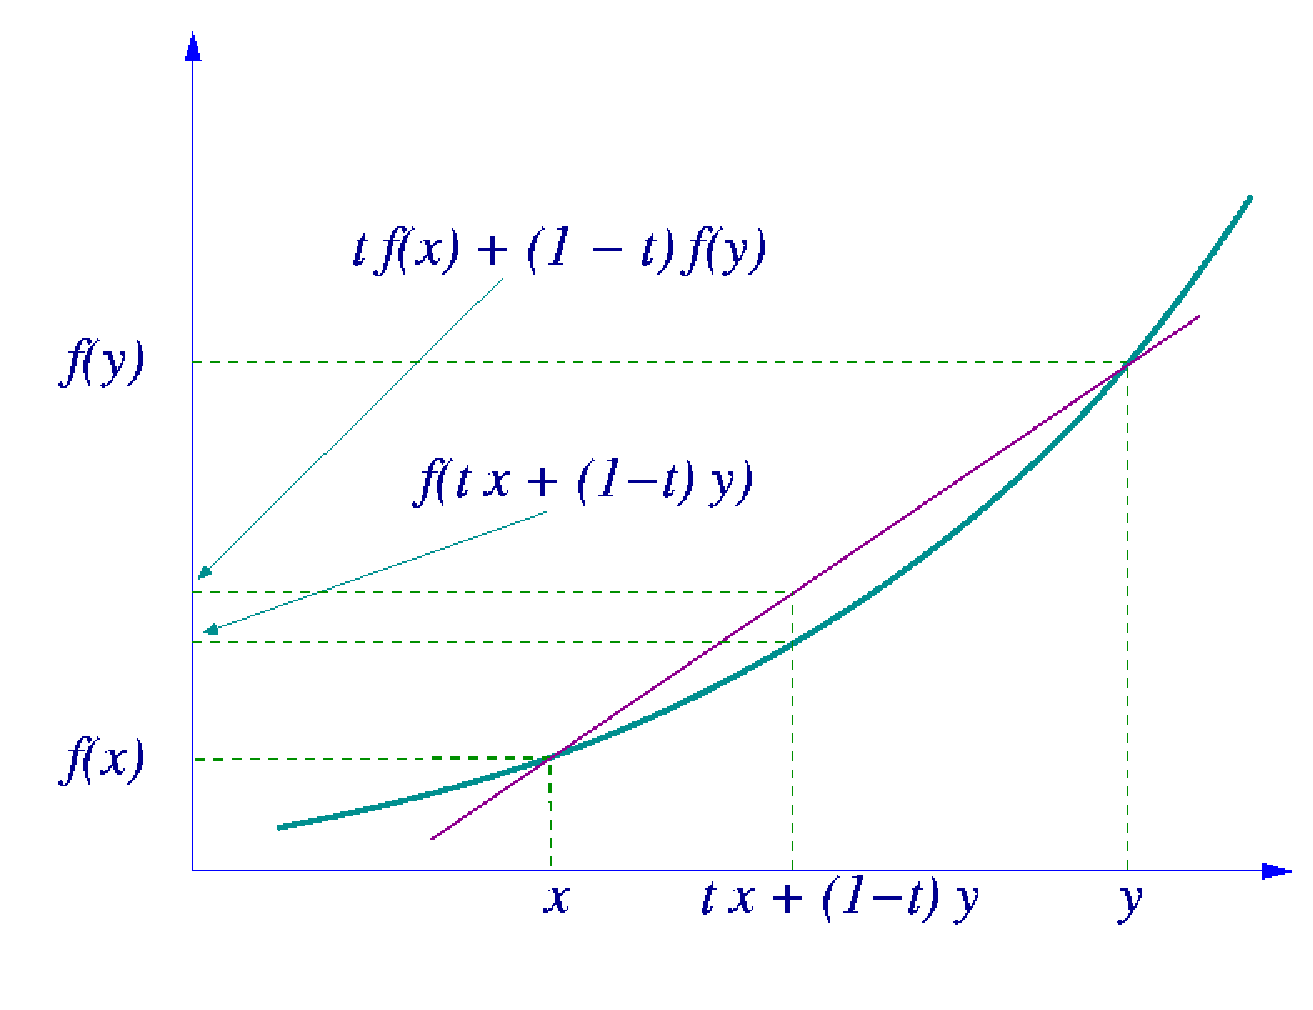
\includegraphics[width=4in]{lecture9/convex.eps}
  \caption{Выпуклая функция}
  \label{fig:convex}
\end{figure}

В доказетельстве неравенства Йенсена используется лемма: для выпуклой функции $f \colon \mathbb{R}\to\mathbb{R}$, $x_1, x_2, \twodots x_n \in \mathbb{R}$ и $\alpha_1, \alpha_2, \twodots \alpha_n \in \mathbb{R}$, $\sum_{k=1}^{n}\alpha_k = 1$, то $f(\sum_{k=1}^{n} \alpha_k x_k) \leqslant \sum_{k=1}^{n} \alpha_k f(x_k)$. Лемма аналогична определению, но для случая $n$ переменных.

Графически видно, что линейная комбинация в левой части уравнения задаёт выпуклый многоугольник, все точки внутри которого лежат выше кривой.

Лемма доказывается по индукции:
\begin{align*}
  f(\sum_{k=1}^{n} \alpha_k x_k) = \text{(по индукционной гипотезе)} \\ 
  = f(a_n x_n + (1-\alpha_n) \sum_{k=1}^{n-1} \frac{a_k}{1-\alpha_n} x_k) = \text{(отделяем меньшую часть)} \\
  \text{т.к. } \alpha_n + (1-\alpha_n) = 1 \text{ и сумма всех } \alpha_k = 1 - \alpha_n \\
  \leqslant \alpha_n f(x_n) + (1-\alpha_n)f(\sum_{k=1}^{n-1} \frac{a_k}{1-\alpha_n} x_k) \leqslant \text{(по свойству выпуклой функции)} \\
  \leqslant \alpha_n f(x_n) + (1-\alpha_n)\sum_{k=1}^{n-1} \frac{a_k}{1-\alpha_n} f(x_k) = \text{(по индукционной гипотезе)} \\
  = \sum_{k=1}^{n} \alpha_k f(x_k) \text{(ч.т.д.)}
\end{align*}

Случай для бесконечного числа переменных $x_n$ доказывается аналогично: от обоих частей уравнения берется предел при $n \to \infty$.

Доказательство неравенства Йенсена: $f(E[X]) \leqslant E[f(X)]$, если $f$ -- выпуклая функция.
\begin{align*}
  f(E[X]) = f(\sum_{x = - \infty}^{\infty} x Pr[X = x]) \leqslant \text{(т.к. сумма вероятностей равна 1)} \\
  \leqslant \sum_{x= - \infty}^{\infty} Pr[X = x] f(x) = \\ 
  = \sum_{y \in range(f)} y \sum_{x = f(x) = y} Pr[X = y] = \\
  = \sum_{y \in range(f)} y Pr[f(X) = y] = \\
  = E[f(X)] \text{(ч.т.д.)}
\end{align*}

\subsection{Ожидаемая высота}

Пусть $X_n$ -- случайная величина высоты рандомизированного BST для $n$ узлов, а $Y_n = 2^X_n$ -- выпуклая функция.

Анализ высоты дерева похож на анализ алгоритма Quicksort в том смысле, что после выбора корня дерева $r$ остальные элементы исходного массива разделяются на две части -- меньшие $r$ (пусть $k$ элементов), которые попадут в левое поддерево и большие $r$ ($n - k - 1$), которые попадут в правое поддерево. Каждое из поддеревьев также является случайным рандомизированным BST, что приводит к рекурсивному анализу алгоритма.

Если корень дерева $r$ имеет ранг $k$, тогда $X_n = 1 + \max(X_{k-1}, X{n-k})$, а $Y_n = 2max(Y_{k-1}, Y_{n-k})$.

Переход с помощью индикаторной случайной величины от совокупности случаев к сумме:
\begin{equation*}
  Z_{nk} = \begin{cases}
      1, \text{если корень имеет ранг } k\\
      0, \text{иначе}
  \end{cases}
\end{equation*}
Очевидно $E[Z_{nk}] = 1 / n$.
\begin{align*}
  Y_n = \sum_{k=1}^{n} Z_{nk} (2max(Y_{k-1}, Y_{n-k})) \\
  E[Y_n] = E[\sum_{k=1}^{n} Z_{nk} (2max(Y_{k-1}, Y_{n-k})) ] = \\
  \text{(по свойству линейности)} \\
  = \sum_{k=1}^{n} E[Z_{nk} (2max(Y_{k-1}, Y_{n-k}))] = \\
  \text{(по независимости случайных величин)} \\
  = 2 \sum_{k=1}^{n} E[Z_{nk}] E[max(Y_{k-1}, Y_{n-k})] = \\
  \text{(т.к. сумма больше максимума)} \\
  \leqslant \frac{2}{n} \sum_{k=1}^{n} E[Y_{k-1} + Y_{n-k}] = \\
  \text{(по свойству линейности)} \\
  = \frac{4}{n}\sum_{k=0}^{n-1}E[Y_k]
\end{align*}
Решаем рекурентность методом подстановки, поставляя $n^3$:
\begin{align*}
  E[Y_n] \leqslant \frac{4}{n}\sum_{k=0}^{n-1}E[Y_k] \leqslant \\
  \leqslant \frac{4}{n}\sum_{k=0}^{n-1}c k^3 \leqslant \\
  \leqslant \frac{4}{n}\int_{0}^{n}x^3 dx = \\
  = \frac{4c}{n} \frac{n^4}{4} = \\
  = c n^3
\end{align*}
В итоге:
\begin{align*}
  E[2^{X_n}] = E[Y_n] = O(n^3) \\
  2^E[X_n] \leqslant E[2^{X_n}] \\
  E[X_n] \leqslant \lg O(n^3) \\
  \text{(константа, присутствующая в O выносится)} \\
  E[X_n] \leqslant 3 \lg n + O(1) \\
\end{align*}

\section{Алгоритмы работы с BST}
Пусть высота бинарного дерева равна $h$. Тогда алгоритм поиска элемента $k$ в дереве с корнем $x$ выполняется за время $O(h)$:
\begin{codebox}
\Procname{$\proc{Tree\_Search}(x, k)$}
\li \If $x = NIL$ | $k = key[x]$
\li \Then \Return $x$
\End
\li \If $k < key[x]$
\li \Then \Return $Tree\_Search(left[x], k)$
\li \Else \Return $Tree\_Search(left[x], k)$
\End
\end{codebox}
Процедуру можно превратить в итеративную с помощью хвостовой рекурсии.

\subsection{Алгоритмы вставки и удаления элемента}
Алгоритм вставки узла $z$, у которого $key[z] = v$, $left[z] = NIL$, $right[z] = NIL$ в дерево $T$:
\begin{codebox}
\Procname{$\proc{Tree\_Insert}(T, z)$}
\li $y \gets NIL$
\li $x \gets root[T]$
\li \While $x \neq NIL$
\li   \Do $y \gets x$
\li     \If $key[z] < key[x]$
\li       \Then $x \gets left[x]$
\li       \Else $x \gets right[x]$
  \End
\End
\li $p[z] \gets y$
\li \If $y = NIL$
\li   \Then $root[T] \gets z$ \Comment Дерево T -- пустое
\li   \Else \If $key[z] < key[y]$
\li       \Then $left[y] \gets z$
\li       \Else $right[y] \gets z$
  \End
\End
\end{codebox}

Цикл в начале процедуры перемещает указатели вниз по дереву в зависимости от сравнения ключей $key[x]$ и $key[z]$, до тех пор, пока $x$ не станет равным NIL. Это значение находится именно в той позиции, куда следует вставить узел $z$.

Процедура Tree\_Delete рассматривает три возможных случая:
\begin{enumerate}
\item Если у узла $z$ нет дочерних узлов, он просто удаляется из дерева
\item Если у узла один дочерний узел, он ``склеивается'' с родительским для $z$
\item Если дочерних узла два, то в дереве находим следующий за $z$ узел $y$, у которого нет левого дочернего узла, убираем его из позиции, где он находился ранее и заменяем им узел $z$
\end{enumerate}

Процедура Tree\_Successor возвращает следующий элемент за аргументом в отсортированной последовательности.

\begin{codebox}
\Procname{$\proc{Tree\_Delete}(T, z)$}
\li \If $left[z] = NIL$ | $right[z] = NIL$
\li   \Then $y \gets z$
\li   \Else $y \gets Tree\_Successor(z)$
  \End
\li \If $left[y] \neq NIL$
\li   \Then $x \gets left[y]$
\li   \Else $x \gets right[y]$
  \End
\li \If $x \neq NIL$
\li   \Then $p[x] \gets p[y]$
  \End
\li \If $p[y] = NIL$
\li   \Then $root[T] \gets x$
\li   \Else \If $y = left[p[y]]$
\li         \Then $left[p[y]] \gets x$
\li         \Else $right[p[y]] \gets x$
  \End
\End
\li \If $y \neq z$
\li   \Then $key[z] \gets key[y]$
\li   \Comment Копирование сопутствующих данных в $z$
  \End
\li \Return $y$
\End
\end{codebox}

Очевидно, что балансировку дерева можно нарушить, вставляя или удаляя специально подобранные элементы. Для борьбы с таким поведением существуют специальные структуры данных и соответствующие алгоритмы: красно-чёрные деревья и AVL-деревья.

\end{document}
